\thispagestyle{fancy}
\vspace*{\fill}
\subsection{Tela comando contagem}
 Esta tela é acessada pelo botão "\textgreater" no menu superior esquerdo da tela de comando dobra, pelo botão "CNT" em qualquer tela de comando e pelo botão comando da tela ajustes contagem.
\begin{figure}[h]
  \centering
  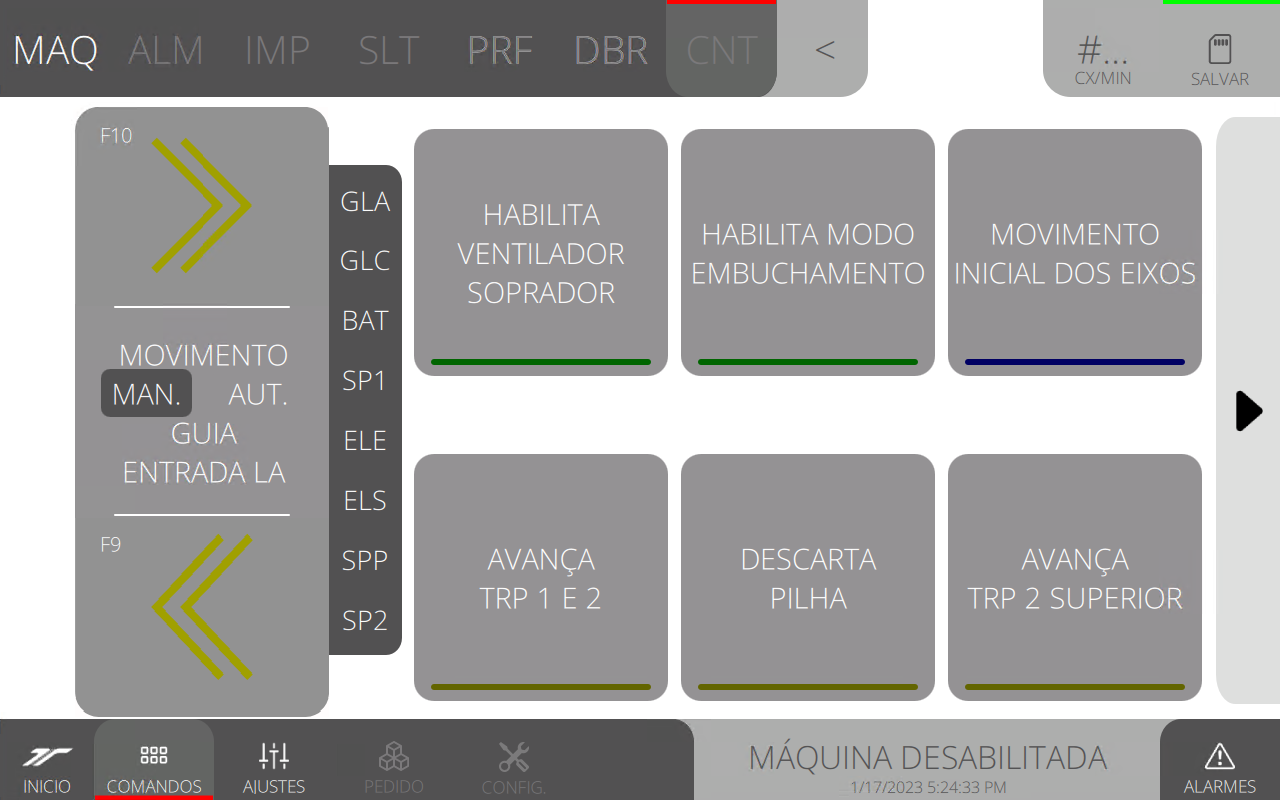
\includegraphics[width=576px,height=360px]{src/imagesFlexo/08-count/commands/e-Tela-Principal.png}
  \caption{ver depois.}
   \label{}
\end{figure}

\newpage
\thispagestyle{fancy}
\vspace*{\fill}
\subsubsection{\small{Menu JOG eixos}}
\begin{figure}[h]
  \centering
  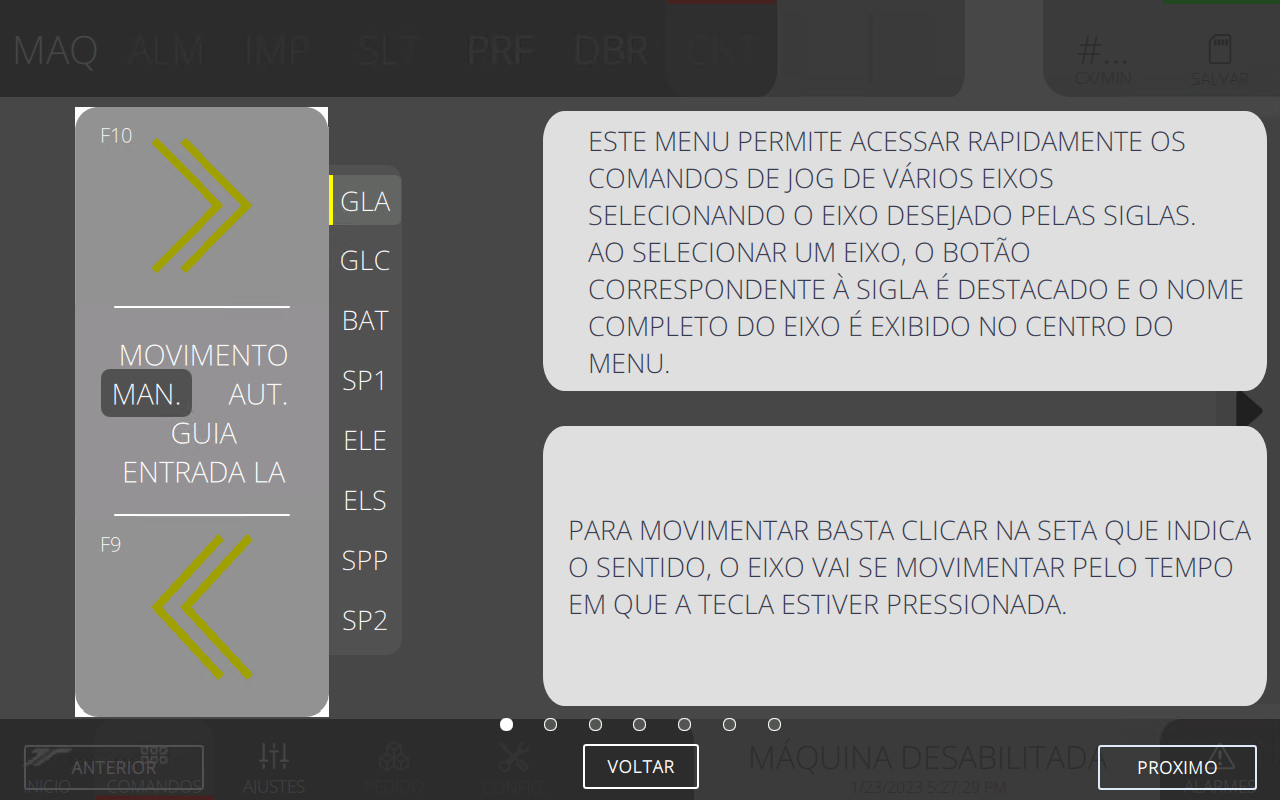
\includegraphics[width=576px,height=360px]{src/imagesFlexo/08-count/commands/e-1.png}
  \caption{ver depois.}
   \label{}
\end{figure}
\vspace*{\fill}

\newpage
\thispagestyle{fancy}
\vspace*{\fill}
\subsubsection{\small{Habilita ventilador soprador}}
\begin{figure}[h]
  \centering
  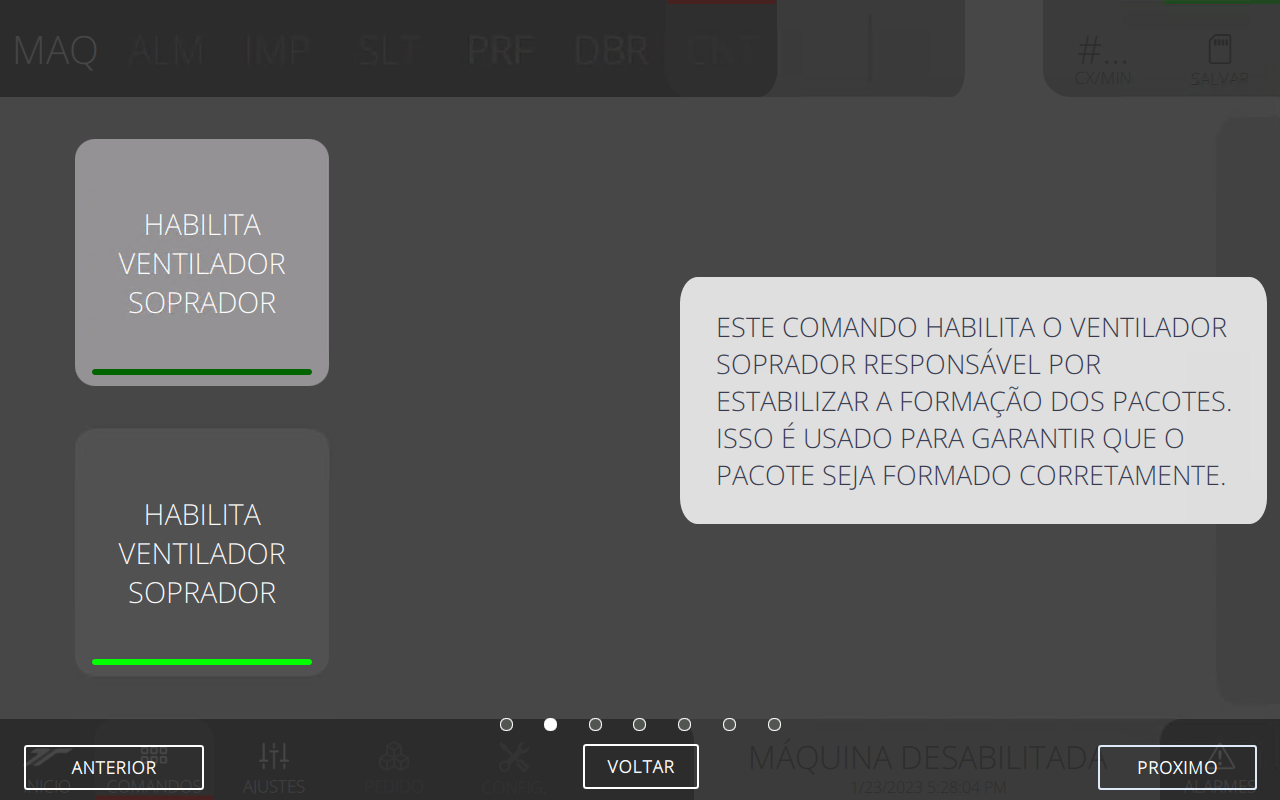
\includegraphics[width=576px,height=360px]{src/imagesFlexo/08-count/commands/e-2.png}
  \caption{ver depois.}
   \label{}
\end{figure}
\vspace*{\fill}

\newpage
\thispagestyle{fancy}
\vspace*{\fill}
\subsubsection{\small{Habilita modo embuchamento}}
\begin{figure}[h]
  \centering
  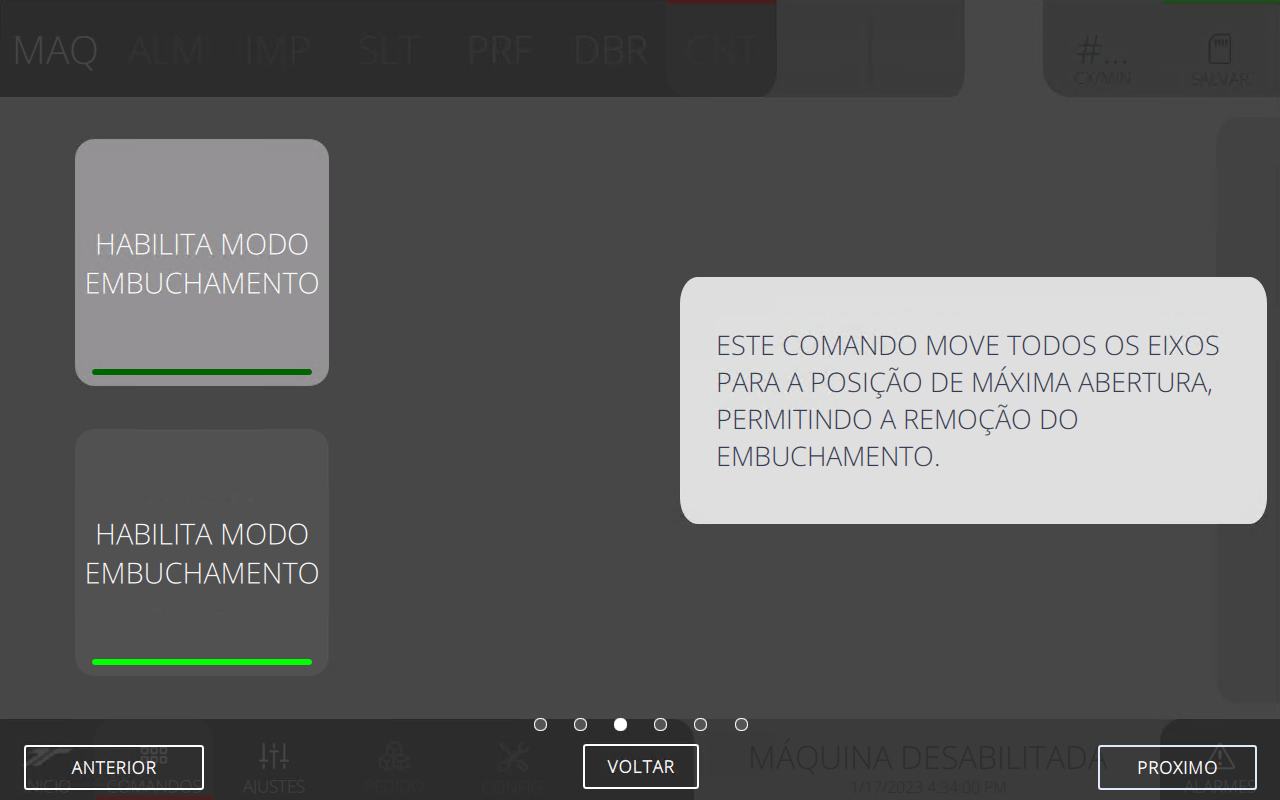
\includegraphics[width=576px,height=360px]{src/imagesFlexo/08-count/commands/e-3.png}
  \caption{ver depois.}
   \label{}
\end{figure}
\vspace*{\fill}

\newpage
\thispagestyle{fancy}
\vspace*{\fill}
\subsubsection{\small{Movimento inicial dos eixos}}
\begin{figure}[h]
  \centering
  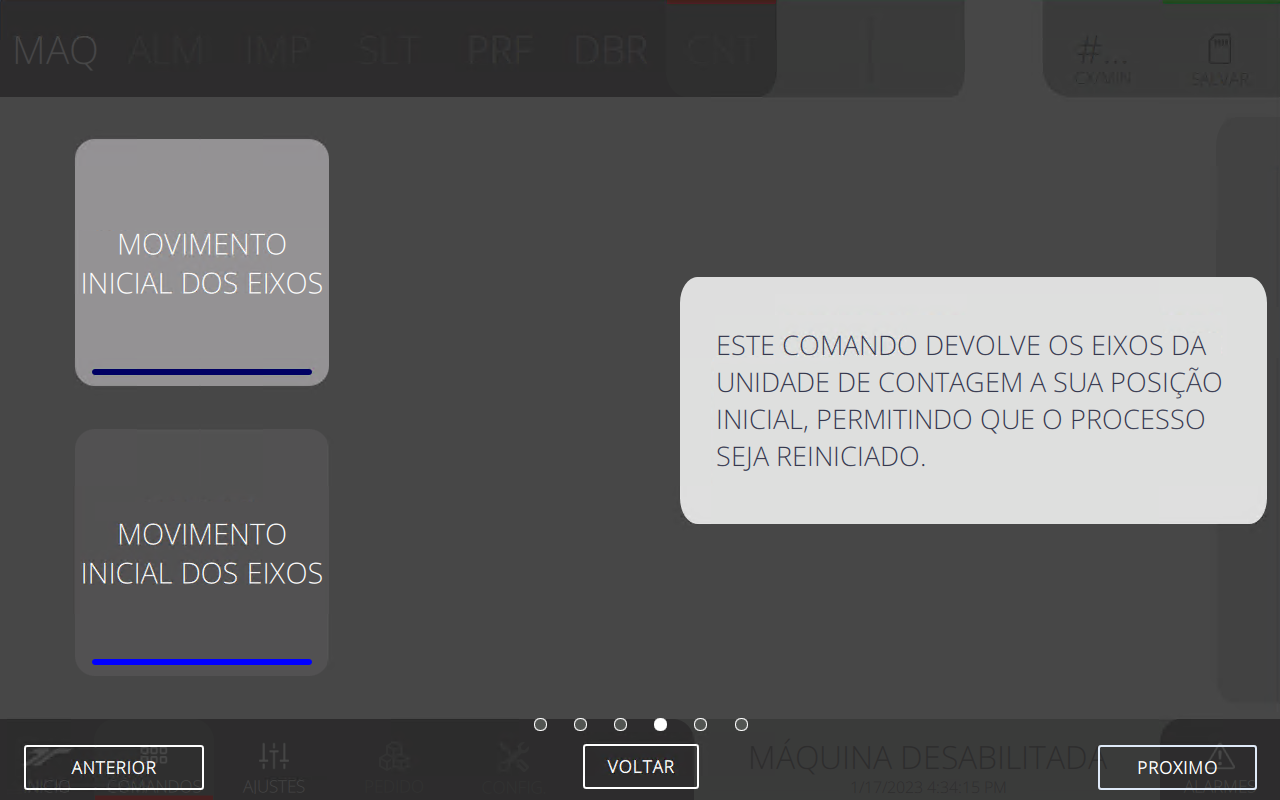
\includegraphics[width=576px,height=360px]{src/imagesFlexo/08-count/commands/e-4.png}
  \caption{ver depois.}
   \label{}
\end{figure}
\vspace*{\fill}

\newpage
\thispagestyle{fancy}
\vspace*{\fill}
\subsubsection{\small{Avança TRP 1 e 2}}
\begin{figure}[h]
  \centering
  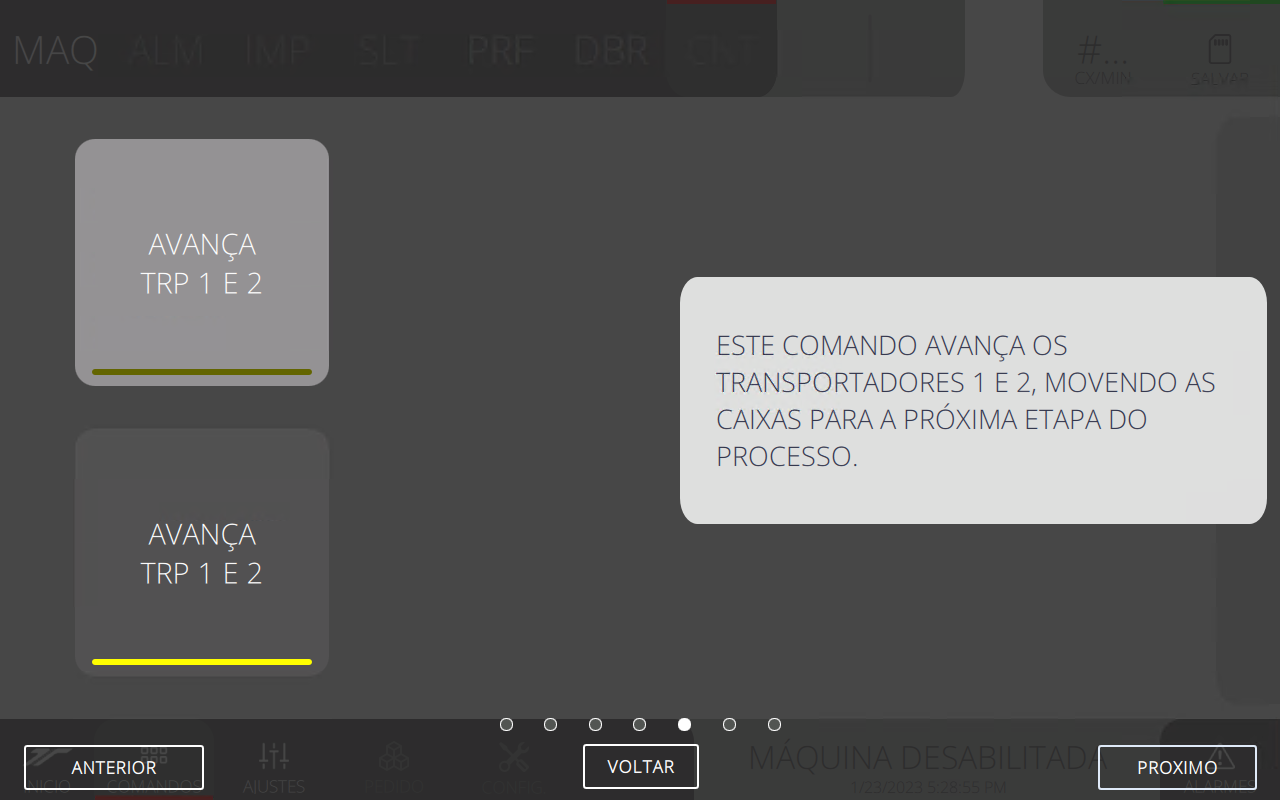
\includegraphics[width=576px,height=360px]{src/imagesFlexo/08-count/commands/e-5.png}
  \caption{ver depois.}
   \label{}
\end{figure}
\vspace*{\fill}

\newpage
\thispagestyle{fancy}
\vspace*{\fill}
\subsubsection{\small{Descarta pilha}}
\begin{figure}[h]
  \centering
  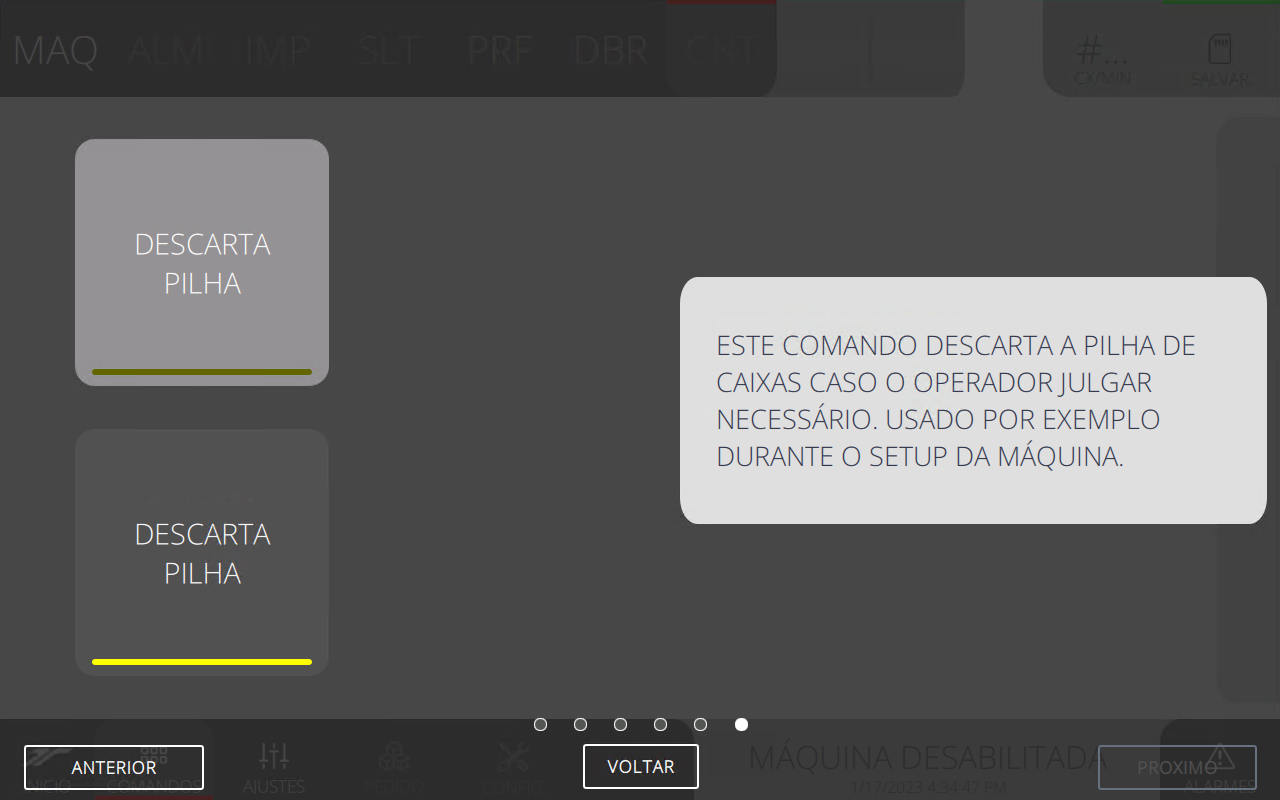
\includegraphics[width=576px,height=360px]{src/imagesFlexo/08-count/commands/e-6.png}
  \caption{ver depois.}
   \label{}
\end{figure}
\vspace*{\fill}

\newpage
\thispagestyle{fancy}
\vspace*{\fill}
\subsubsection{\small{Avança TRP 2 superior}}
\begin{figure}[h]
  \centering
  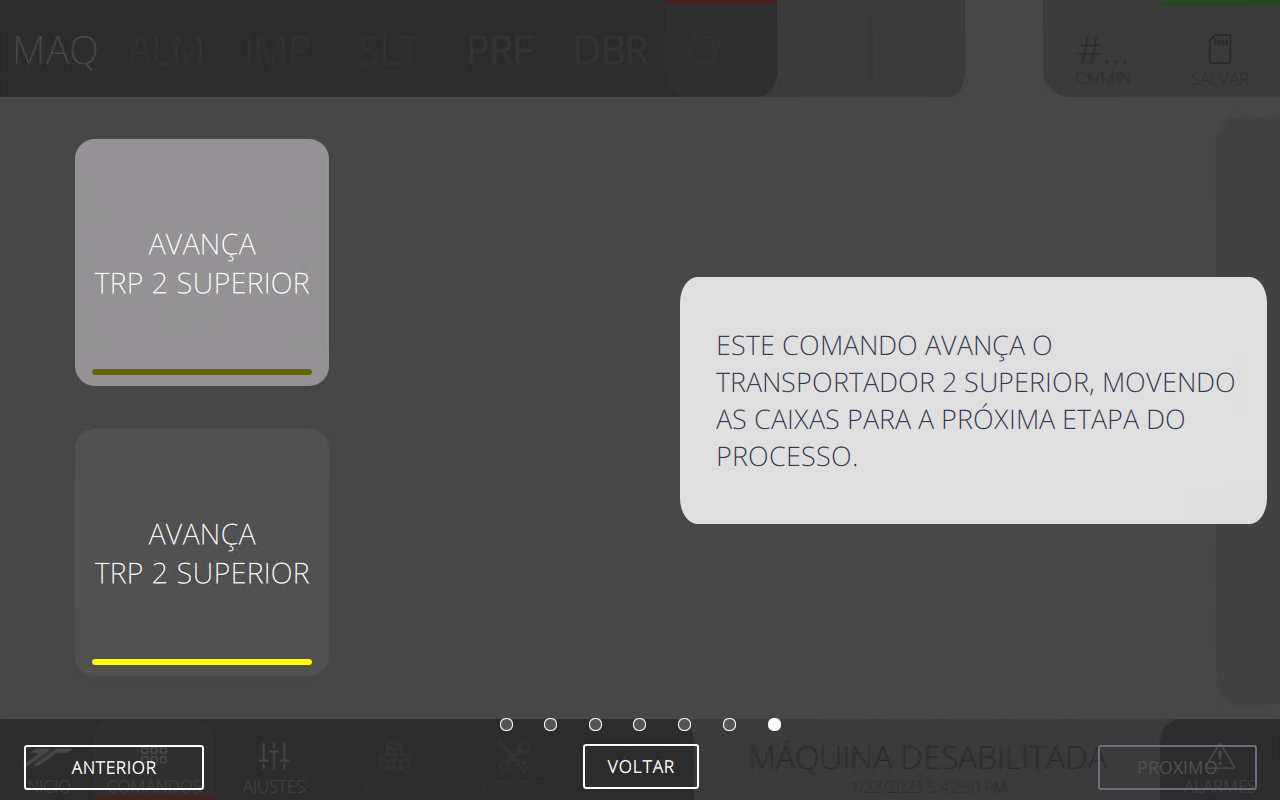
\includegraphics[width=576px,height=360px]{src/imagesFlexo/08-count/commands/e-7.png}
  \caption{ver depois.}
   \label{}
\end{figure}
\vspace*{\fill}

\newpage
\thispagestyle{fancy}
\vspace*{\fill}
\subsection{Segunda tela comando contagem}
Esta tela é acessada pelo botão direito "\textgreater" na tela de comando contagem. A lógica dos outros menus continua sendo a mesma da sua tela "pai" e para voltar a tela anterior basta clicar no botão esquerdo "\textless{}".
\begin{figure}[h]
  \centering
  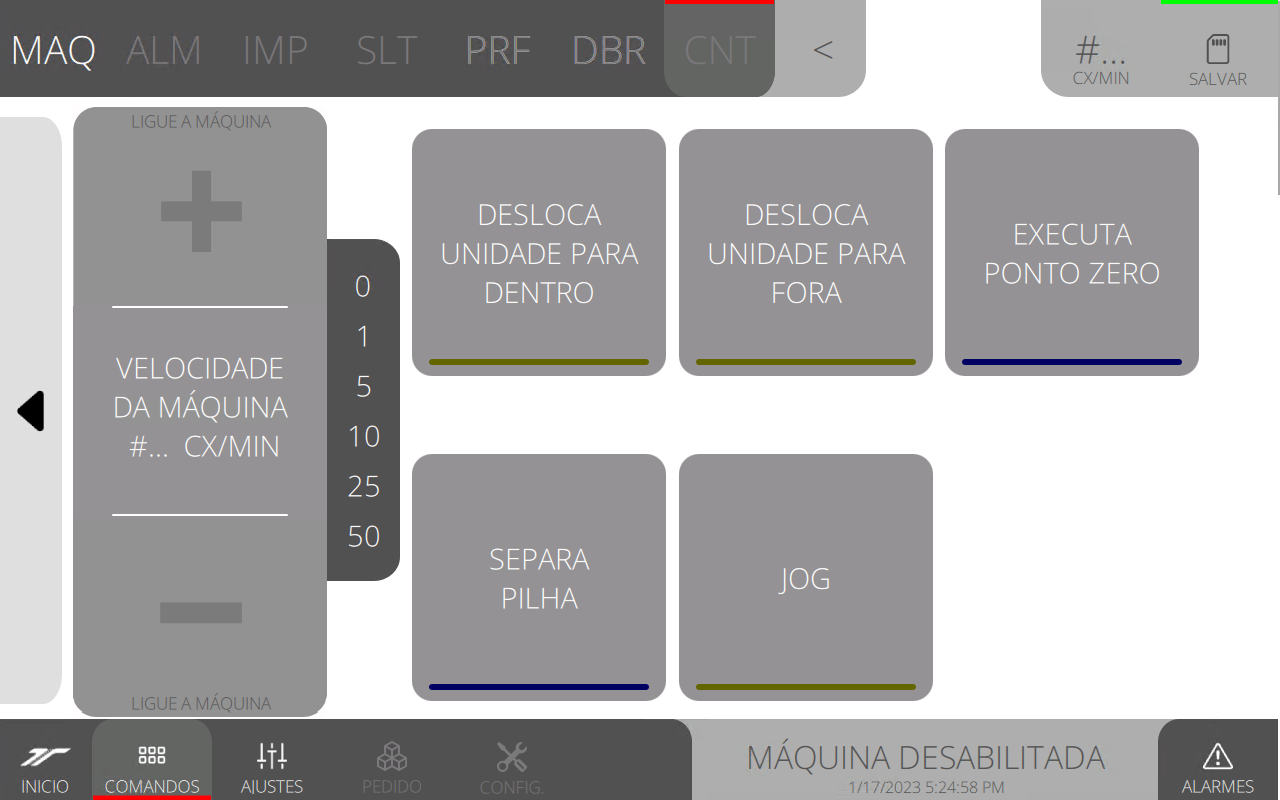
\includegraphics[width=576px,height=360px]{src/imagesFlexo/08-count/commands/e-Tela-Principal-2.png}
  \caption{ver depois.}
   \label{}
\end{figure}

\newpage
\thispagestyle{fancy}
\vspace*{\fill}
\subsubsection{\small{Desloca unidade para dentro}}
\begin{figure}[h]
  \centering
  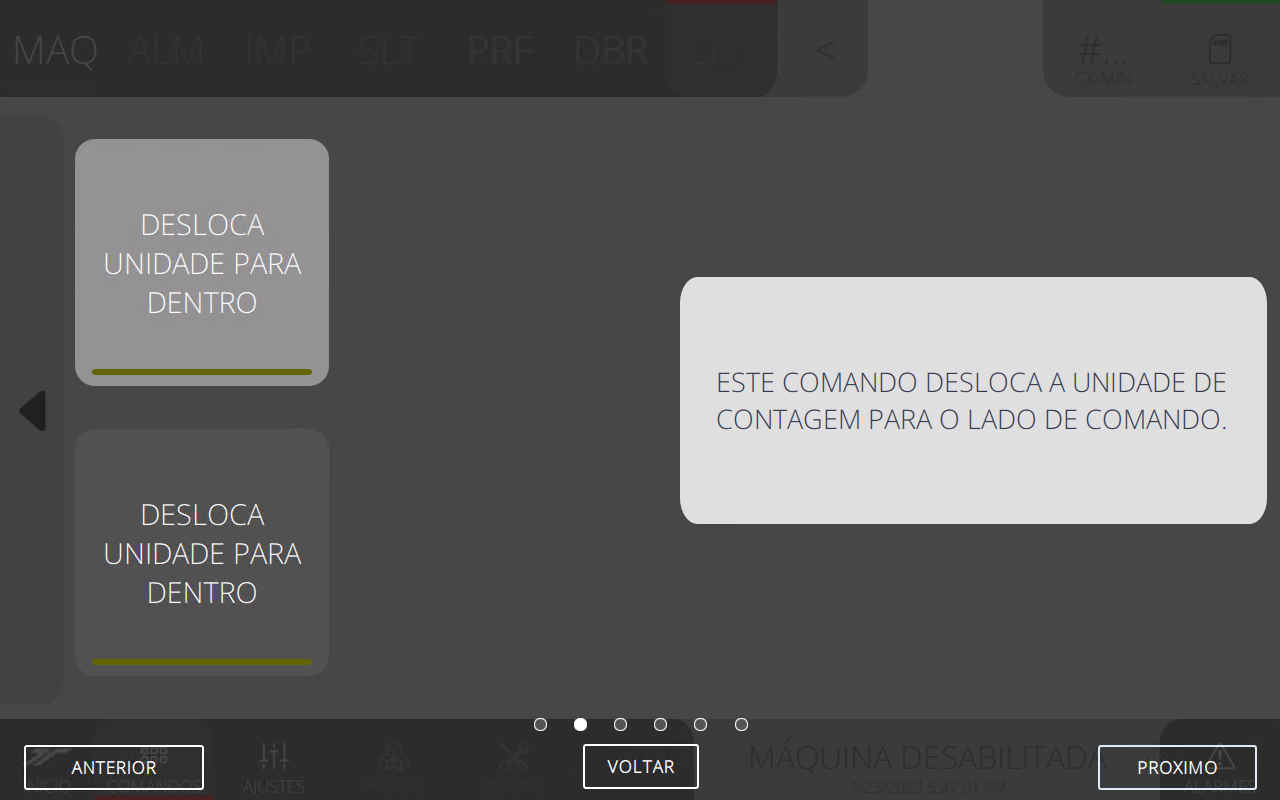
\includegraphics[width=576px,height=360px]{src/imagesFlexo/08-count/commands/e-9.png}
  \caption{ver depois.}
   \label{}
\end{figure}
\vspace*{\fill}

\newpage
\thispagestyle{fancy}
\vspace*{\fill}
\subsubsection{\small{Desloca unidade para fora}}
\begin{figure}[h]
  \centering
  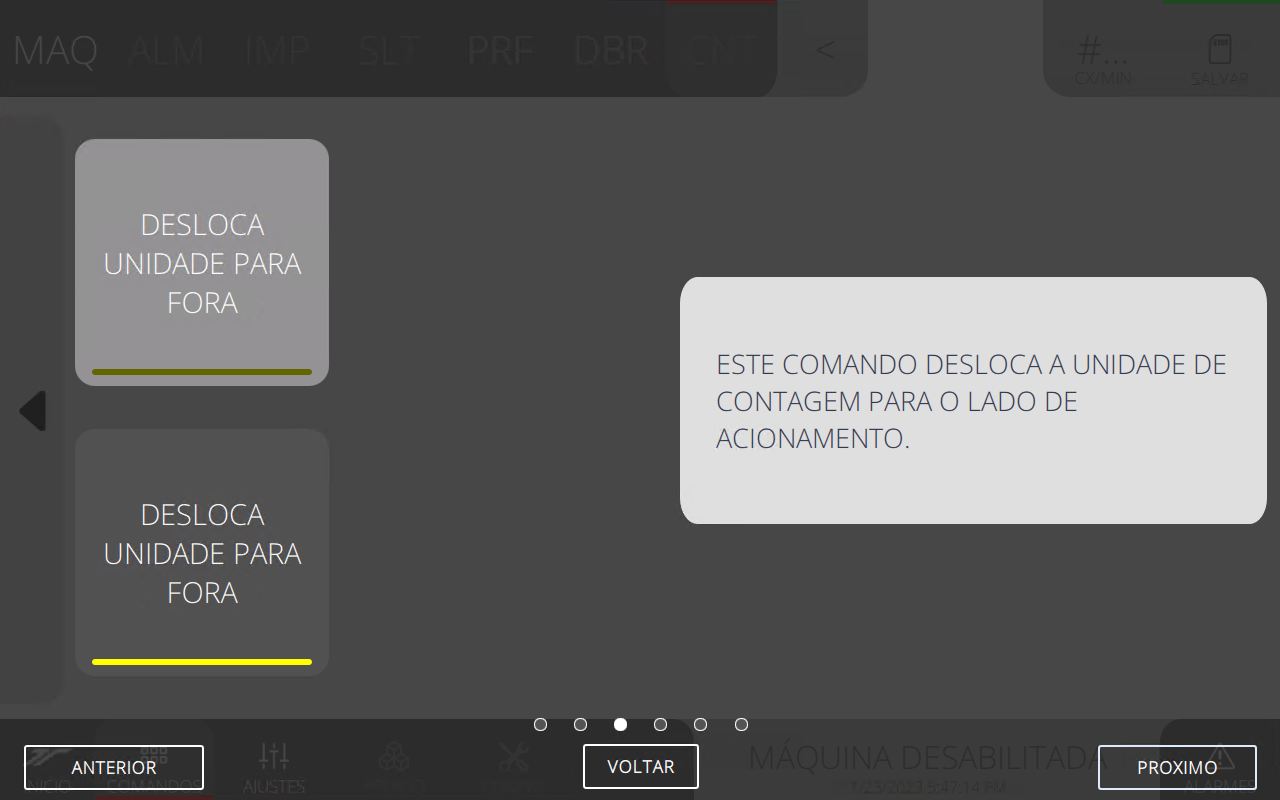
\includegraphics[width=576px,height=360px]{src/imagesFlexo/08-count/commands/e-10.png}
  \caption{ver depois.}
   \label{}
\end{figure}
\vspace*{\fill}

\newpage
\thispagestyle{fancy}
\vspace*{\fill}
\subsubsection{\small{Executa ponto zero}}
\begin{figure}[h]
  \centering
  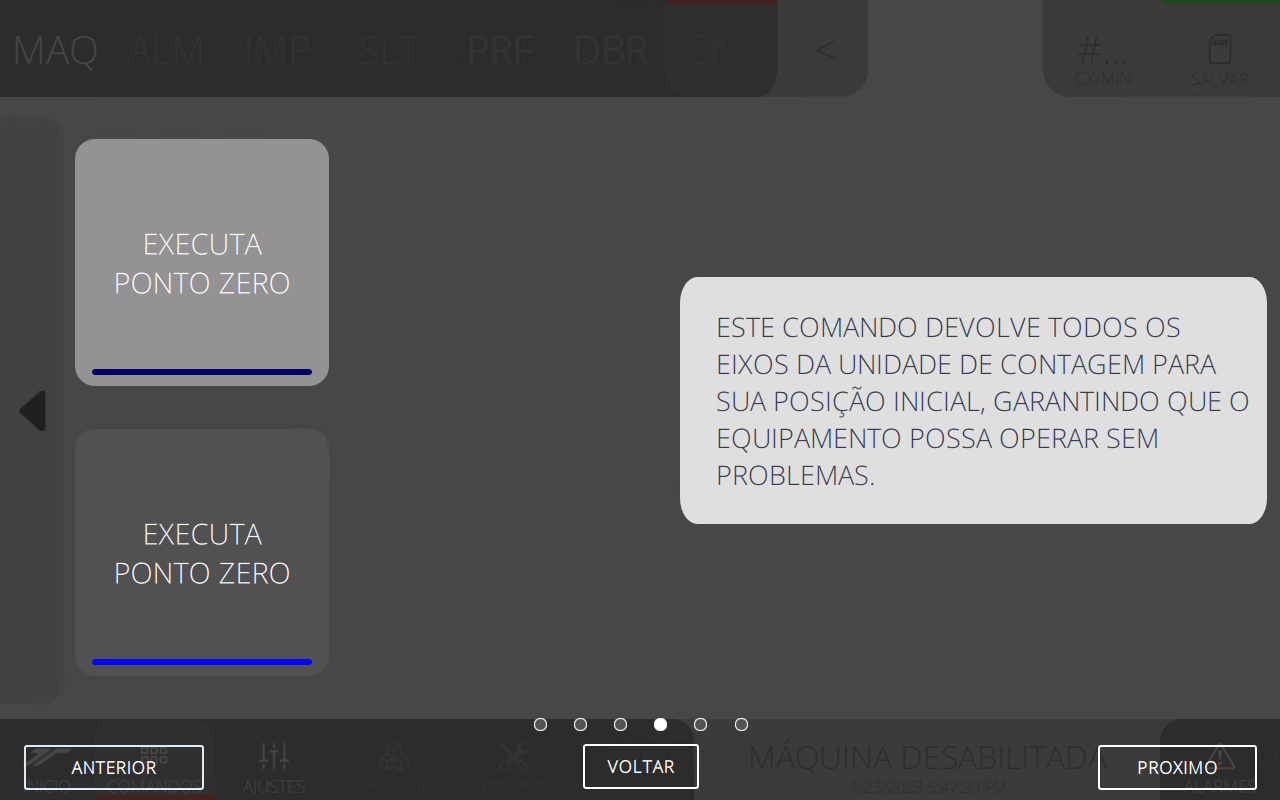
\includegraphics[width=576px,height=360px]{src/imagesFlexo/08-count/commands/e-11.png}
  \caption{ver depois.}
   \label{}
\end{figure}
\vspace*{\fill}

\newpage
\thispagestyle{fancy}
\vspace*{\fill}
\subsubsection{\small{Separa pilha}}
\begin{figure}[h]
  \centering
  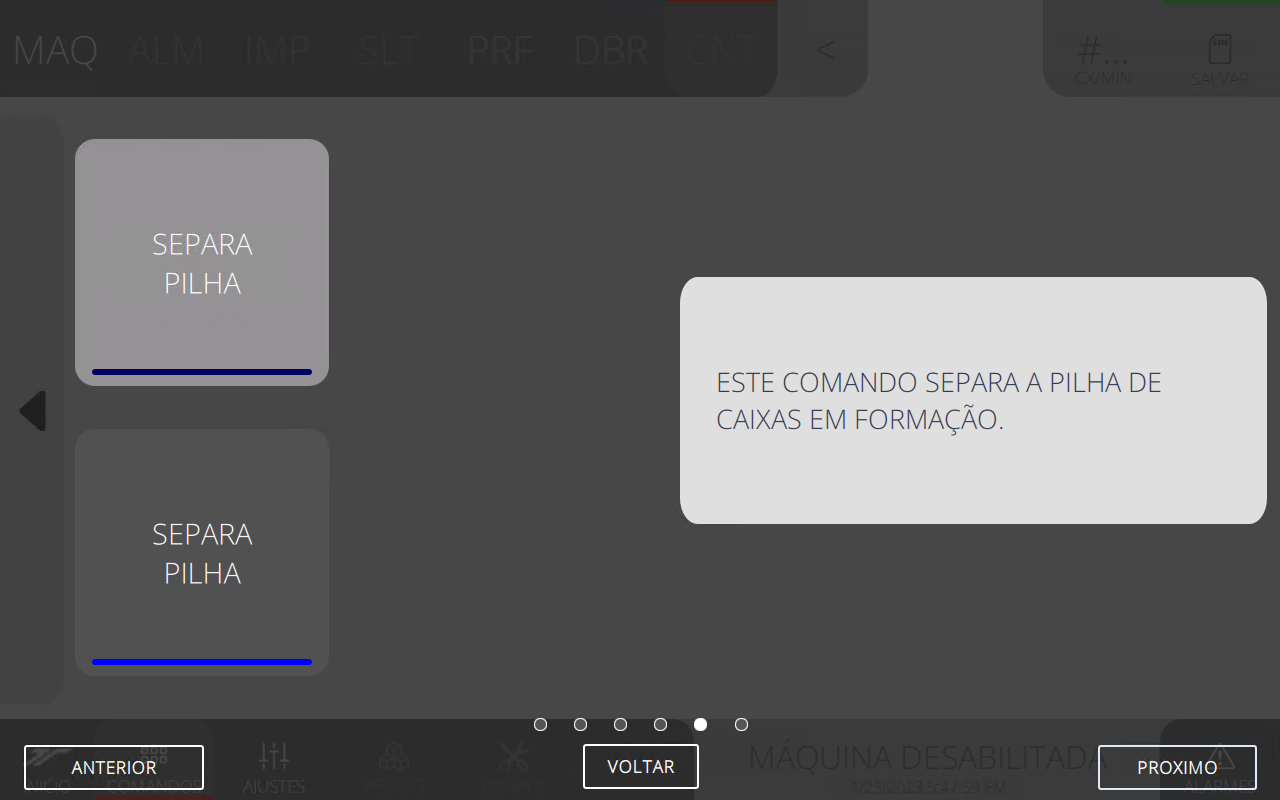
\includegraphics[width=576px,height=360px]{src/imagesFlexo/08-count/commands/e-12.png}
  \caption{ver depois.}
   \label{}
\end{figure}
\vspace*{\fill}

\newpage
\thispagestyle{fancy}
\vspace*{\fill}
\subsubsection{\small{JOG}}
\begin{figure}[h]
  \centering
  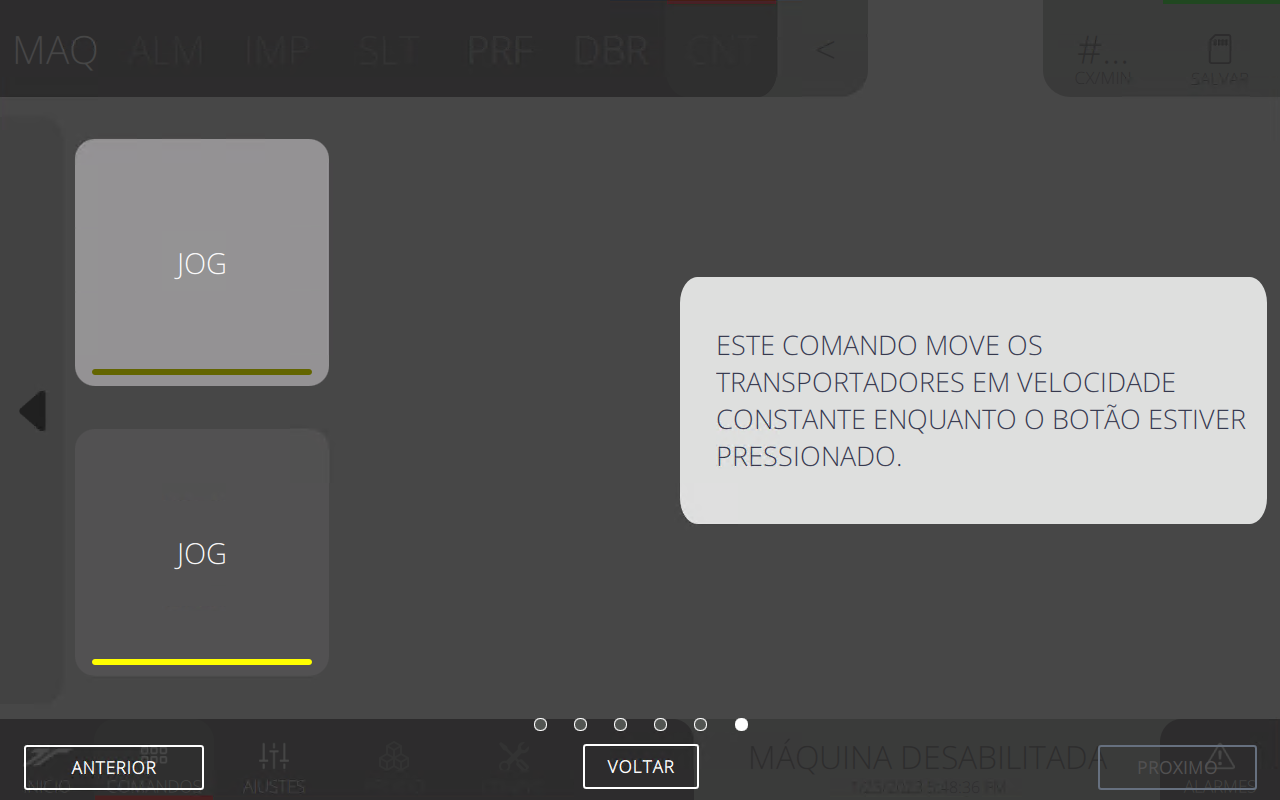
\includegraphics[width=576px,height=360px]{src/imagesFlexo/08-count/commands/e-13.png}
  \caption{ver depois.}
   \label{}
\end{figure}
\vspace*{\fill}